% Part 1:
% - What is P2P?
%   P2P vs client/server
%   Internet/Network
% - History
% - Why P2P?
%   Phylosophy of P2P
%   P2P users/communities

\section{General purpose}

  \begin{frame}
    \tableofcontents[currentsection, hideothersubsections]
  \end{frame}

  % What is P2P?
  \subsection{What is P2P?}
    \begin{frame}
      \frametitle{P2P vs client/server}
      \framesubtitle{Two distinct models}
      \begin{figure}
        \hfill
        \subfigure[Centralized network]{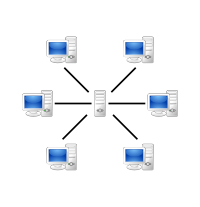
\includegraphics[scale=0.5]{img/P1-client-server.png}}
        \hfill
        \subfigure[P2P network]{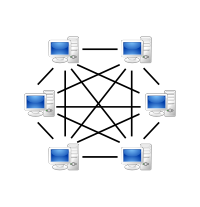
\includegraphics[scale=0.5]{img/P1-p2p.png}}
        \hfill
        \caption{Network architectures}
      \end{figure}
    \end{frame}
    
    \begin{frame}
      \frametitle{P2P network paradigm}
      \framesubtitle{What, where, who, how?}
      \begin{enumerate}
      \item[What] : P2P is a protocol that allows resource sharing.
      \item[Where] : resources are hosted by clients.
      \item[Who] : clients = servers = users.
      \item[How] : users are connected to one another using a software.
      \end{enumerate}
    \end{frame}
    
  % History
  \subsection{History}
    \begin{frame}
      \frametitle{Overview}
      \framesubtitle{It all began when...}
      \begin{figure}
        \centering
        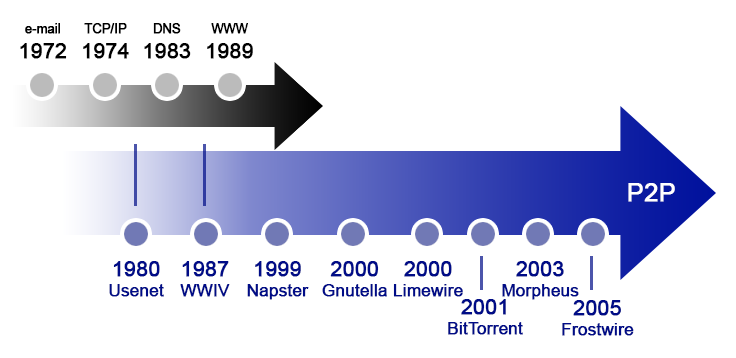
\includegraphics[scale=1.5]{img/P1-time.png}
        \caption{P2P timeline}
      \end{figure}
    \end{frame}
    
    \begin{frame}
      \frametitle{Main stages}
      \framesubtitle{1980 > 2001}
      \begin{enumerate}
      \item[1980] Usenet : first decentralized resources system.
      \item[1997] Napster : centralized search mechanisms, files hosted by users.
      \item[2000] Gnutella : decentralized searching, routing and hosting.
      \item[2001] BitTorrent : decentralized resources, splited into subnetworks.
      \end{enumerate}
      \begin{figure}
        \hfill
        \subfigure[Napster]{
\includegraphics[scale=0.17]{img/P1-napster.png}}
        \hfill
        \subfigure[Gnutella]{
\includegraphics[scale=0.2]{img/P1-gnutella.png}}
        \hfill
        \subfigure[BitTorrent]{
\includegraphics[scale=0.215]{img/P1-bittorrent.png}}
        \hfill
        \caption{P2P Softwares}
      \end{figure}
    \end{frame}
    
  % Why use P2P?
  \subsection{Why using P2P?}
    \begin{frame}
      \frametitle{Philosophy of P2P}
      \framesubtitle{"Delivering the World's Content"}
      \begin{enumerate}
      \item[-] Big Brother can not watch you.
      \item[-] Everyone pulls their own weight.
      \item[-] Peers have the same privileges and rights.
      \item[-] Everyone can request for resources as well as grant them.
      \item[-] Users communicate with each other directly.
      \item[-] Communities help people to find their way.
      \end{enumerate}
    \end{frame}
    
    \begin{frame}
      \frametitle{Communities}
      \framesubtitle{Who's delivering content?}
      Various lists of available content (legal or not) are released by trackers, mainly accessible through the BitTorrent protocol.\\
      Your job is to choose wisely.
      \begin{figure}
        \hfill
        \subfigure[The Pirate Bay]{
\includegraphics[scale=0.08]{img/P1-tpb.png}}
        \hfill
        \subfigure[ClearBits]{
\includegraphics[scale=0.4]{img/P1-clearbits.png}}
        \hfill
        \caption{Illegal(?) and legal trackers}
      \end{figure}
    \end{frame}
